%%% -*-LaTeX-*-

\chapter{Results}

In this chapter we evaluate our system using both labeled and unlabeled data. Our experiments in this section are conducted on a ubuntu16 virtual machine with 80 GB memory and 20 cpus of computing power. 

\section{Dataset: description and clustering}
The traffic analyzed here is collected at the University of Utah's emulab routers \cite{White+:osdi02}. This is a private repository that contains traces of bidirectional traffic into the emulab network and no payload. Traffic is collected on full duplex links at a speed of 1Gbps.

We passed the NetFlow records collected over the last six months of 2017 through our system to determine the set of behaviors hosts exhibited over this time. We have hand picked 7 days of this data for analysis. The chosen days are October 15, October 16, November 14, November 23, December 5, December 12, December 16\footnote{Days are picked without any prior knowledge of any metadata related to NetFlow records}. We made sure that there is a mix of both week days , weekends, normal and heavy traffic days. Each days traffic is treated independently as the same host that appeared on two different days could exhibit different behaviors. For different evaluations in this section we used the data corresponding to the these days.

As mentioned earlier in the section \ref{cluster_labeling} we have choosen a reference day for labeling the clusters. We applied following techniques to label the clusters on the reference day. The first one is port-based analysis to identify applications such as web, mail, and DNS. second one is the anomaly detection methods. Finally, a set of heuristic rules to label manually the behavior of the hosts. After the above steps we found the following clusters. Clusters labeled as T consists of hosts which use few ports on both sides to exchange interactive traffic. Clusters labeled as S consists of hosts which serve clients requests and conversely clusters labeled C consists of hosts which request servers for information. Let us list the differences in these behaviors in detail.

\textbf{Clusters T1-T2} are mostly one-to-one connections, the dominant traffic in these clusters is http/https, ssh and peer to peer traffic. P2P traffic is defined as traffic where hosts uses both TCP and UDP ports concurrently for communication, They also choose arbitary ports for communication. Further analysis, reveals that clusters are split based on packet size and flow size.
While T1 has long living flows with large average packet sizes. T2 has large number of flows which are short lived and an average packet size less than T1.

\textbf{Clusters C1-C2} contains hosts which behave as clients  making connections with different servers, The cluster C2 is dominated by DNS traffic which is in accordance with the heavy DNS requests that the hosts residing in the emulab network make with the external servers (machines outside the Emulab Firewall). Cluster C1 on the other hand comprises of hosts that request for web pages and that have outbound mail traffic.

\textbf{Clusters S1-S2} as mentioned above comprises of hosts that behave as servers which respond to client requests. These hosts generally communicate with different ports of destination machines from a fixed port. S1 cluster contains of majority of hosts which are within emulab network and are acting as servers accepting SSH requests. S2 cluster contains hosts that are both within and outside emulab network which are acting as servers for different sets of traffic such as SSH, Web and DNS which is further explained in the section \ref{cross_validation}. 

\textbf{Cluster A1} is the cluster that is of interest for network security as it contains of hosts that exhibit anamolous behavior trying to scan different access points to enter into the system.

The above description clearly points out that host based behavior extraction produces a richer and finer classification of host behaviors than a port based classifier. For example, Http traffic is split across different clusters T or S which represents how the same protocol can be used by hosts exhibiting different behaviors. Same is the case with SSH traffic. While most of these clusters contain hosts using different protocols. They are similar in the sense that each cluster exhibits different functional behavior such as Server, Client or One-to-One traffic.

We further examined the clusters to determine if there is any similarity in the way the clusters T1/T2 , C1/C2 and S1/S2 are formed. While we found that the clusters T1/T2 are distinguished by average byte size with hosts in T1 having an average byte size higher than hosts in the cluster T1, there were no such features that uniquely defined C1/C2 , S1/S2. This verifies the our system is not biased by any single feature.

\begin{figure}[t]
	\centerline{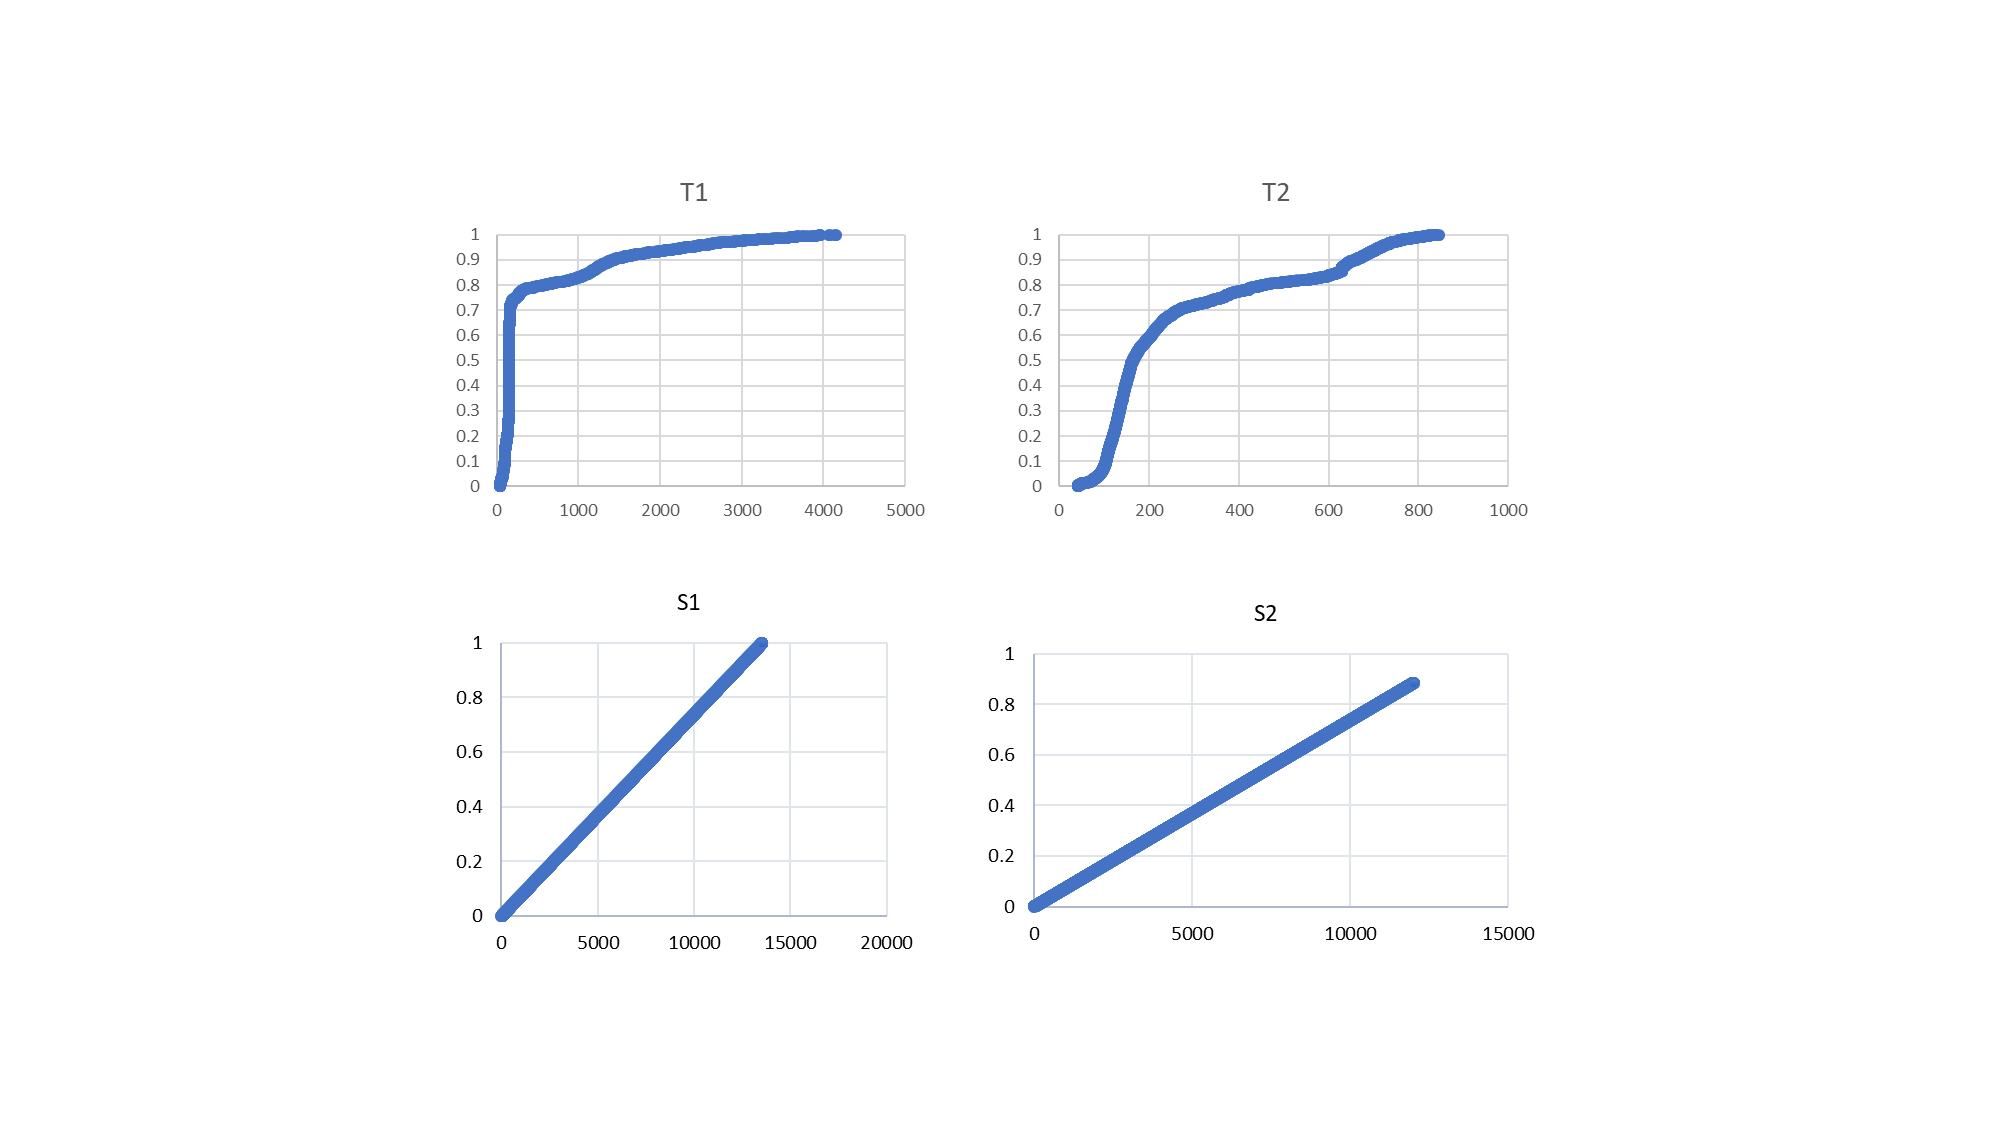
\includegraphics[trim=2cm 2cm 2cm 2cm, scale = 0.7]{bytes_cdf.pdf}}
	\caption{ Average Bytes feature CDF for clusters T1,T2,S1,S2}%
	\figlabel{bytes_cdf}
\end{figure}




The \figref{behaviorsdec12} is a comparison between the classification made by a traditional port based classifer 6.1(a) and our host based classifier 6.1(b). The traditional port based classifier identified the top 8 applications used by the hosts in the system. DNS(53) is the most used application with 11.95\% of the whole traffic trying to query DNS servers. It is followed by Telnet(23), SSH(22) with a share of 9.83\% and 5.08\% traffic respectively. We can also see web traffic both secured and unsecured in the top 8 accounting to 3.84\%, 0.66\% traffic. While, we can see the applications that accounted to majority of traffic by traditional classifier, Our system on the other hand provided an alternate view for the same NetFlow data by extracting the behaviors these hosts are exhibting. From the \figref{behaviorsdec12} we can see that, hosts that are behaving as clients account to 11.41\% (both C1 and C2 combined) of traffic and hosts that are behaving as servers account to 33.61\% (both S1 and S2 combined). The majority of the traffic(50.23\%) comprises of interactive communication between hosts while the anomalous hosts trying to invade into the network form the minority(4.75\%). 

\begin{figure}[t]
	\centerline{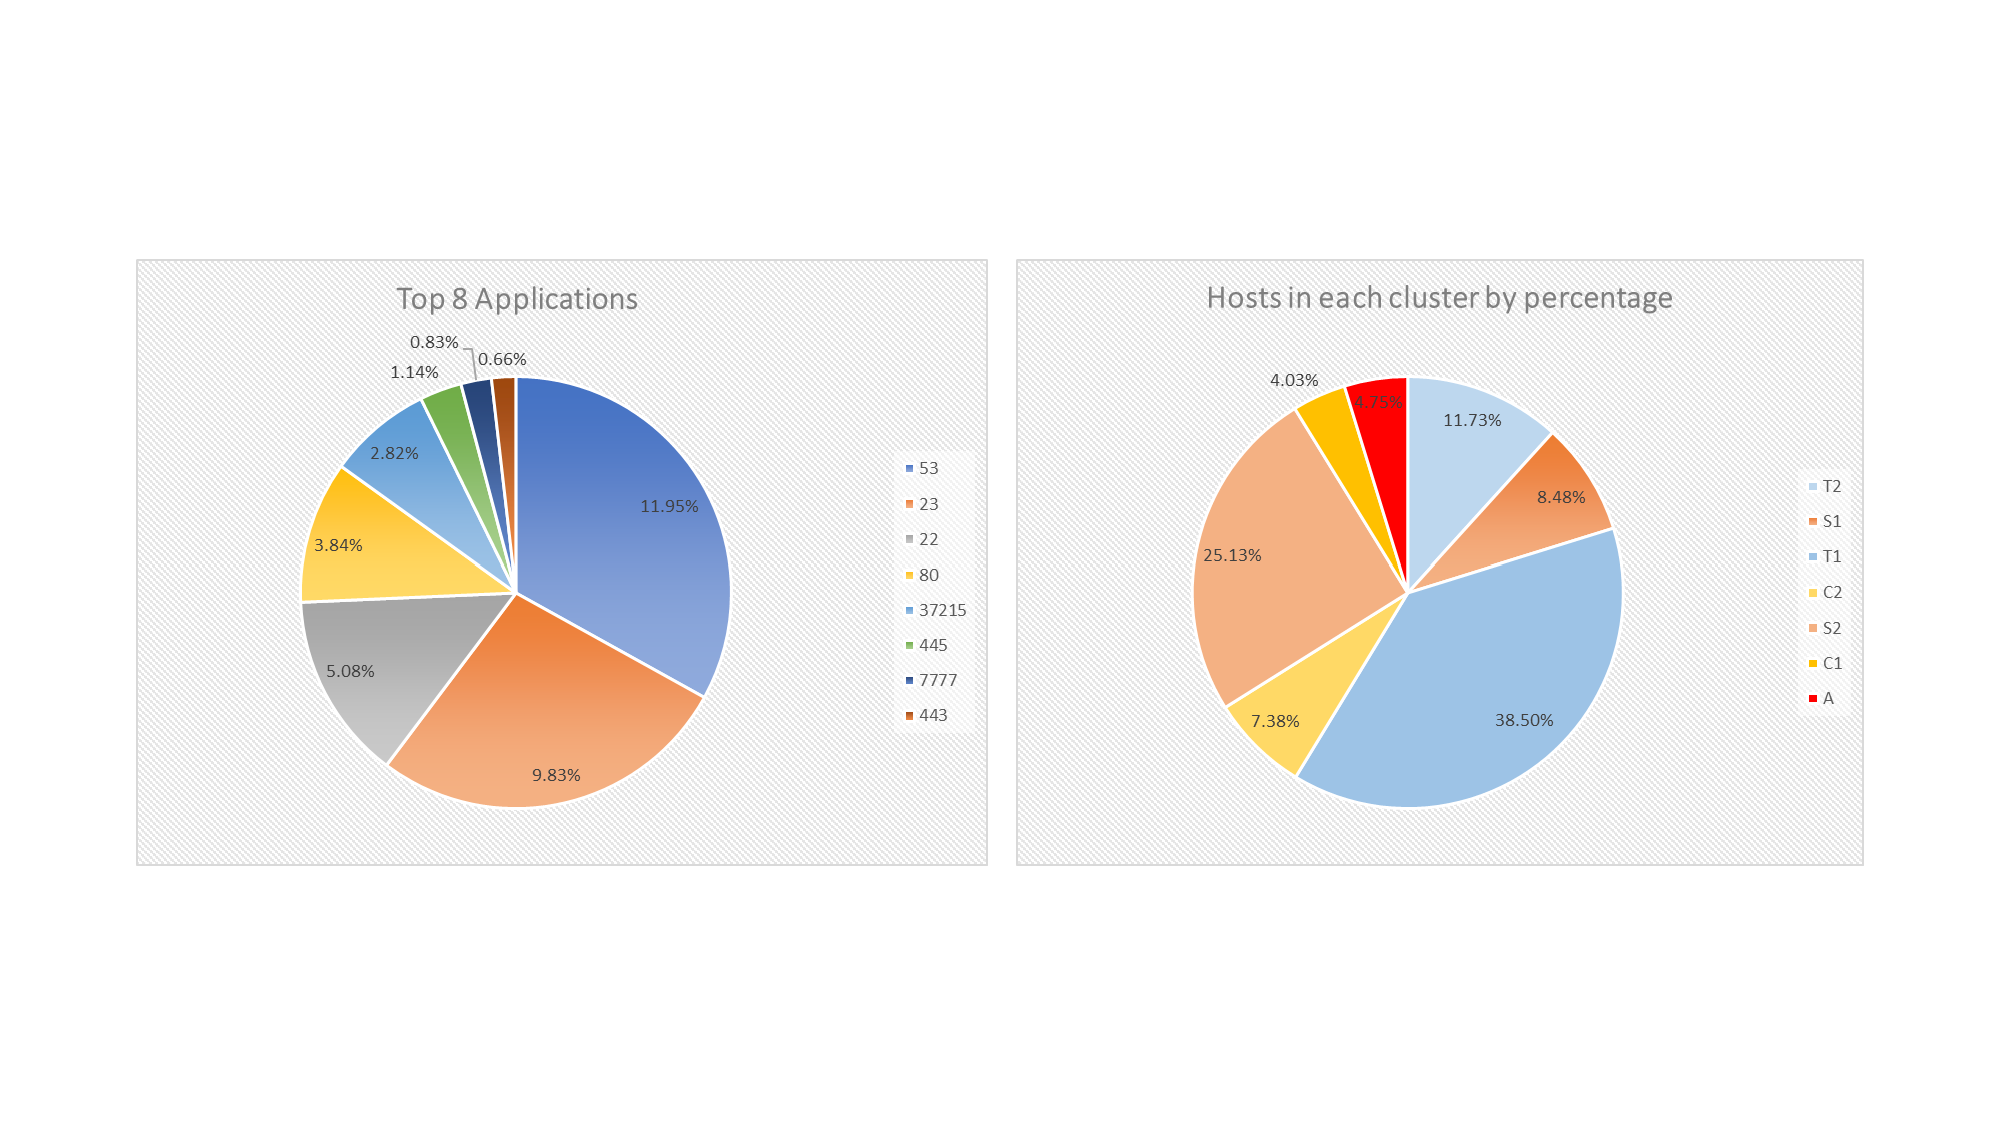
\includegraphics[trim=2cm 2cm 2cm 2cm, scale = 0.5]{dec12-port-behaviors.pdf}}
	\caption{Comparison of hosts using port based classifier (left) and host behavior extractor (right) on December 12, 2017.}%
	\figlabel{behaviorsdec12}
\end{figure}


\section{Cross Validation} \label{cross_validation}
We compared the results obtained from our system with other classification techniques to better understand the significance of our approach.

\textbf{\textit{Cross Validation with a port based classifier}}, We used a classic port based classifying technique to cross validate our results. Though, it isn't a perfect measure and fails in many cases it is good enough to classify a host to a particular class in most of the cases.
In the scenarios when this technique cannot classify a host to particular class we label it as a 'Mix' traffic. The heuristic that we used for labeling as 'Mix' traffic is when the dominant class accounts for less than 50 percent of the traffic by that host. Applying this procedure we observed 20 different classes of traffic, out of which the most frequently observed are discussed here: HTTP, DNS, SSH, MAIL, TELNET, FTP, CHAT, SCAN, SMTP, MIX. Most of these classes are self explanatory based on the ports they operate. SCAN is a class that is different from others while all the other classes deal with single port SCAN deals with multiple ports. A host falls under SCAN category if majority of its traffic is trying to hit multiple ports on a system trying to find an open port to infiltrate. The cross-validation between the port based approach and  our procedure on one of the choosen day December 12th is reported in \tabref{validation}.

\begin{table}[b]
	\caption{Cross-valdation of the host behavior extraction with port based analysis.}%
	\centerline{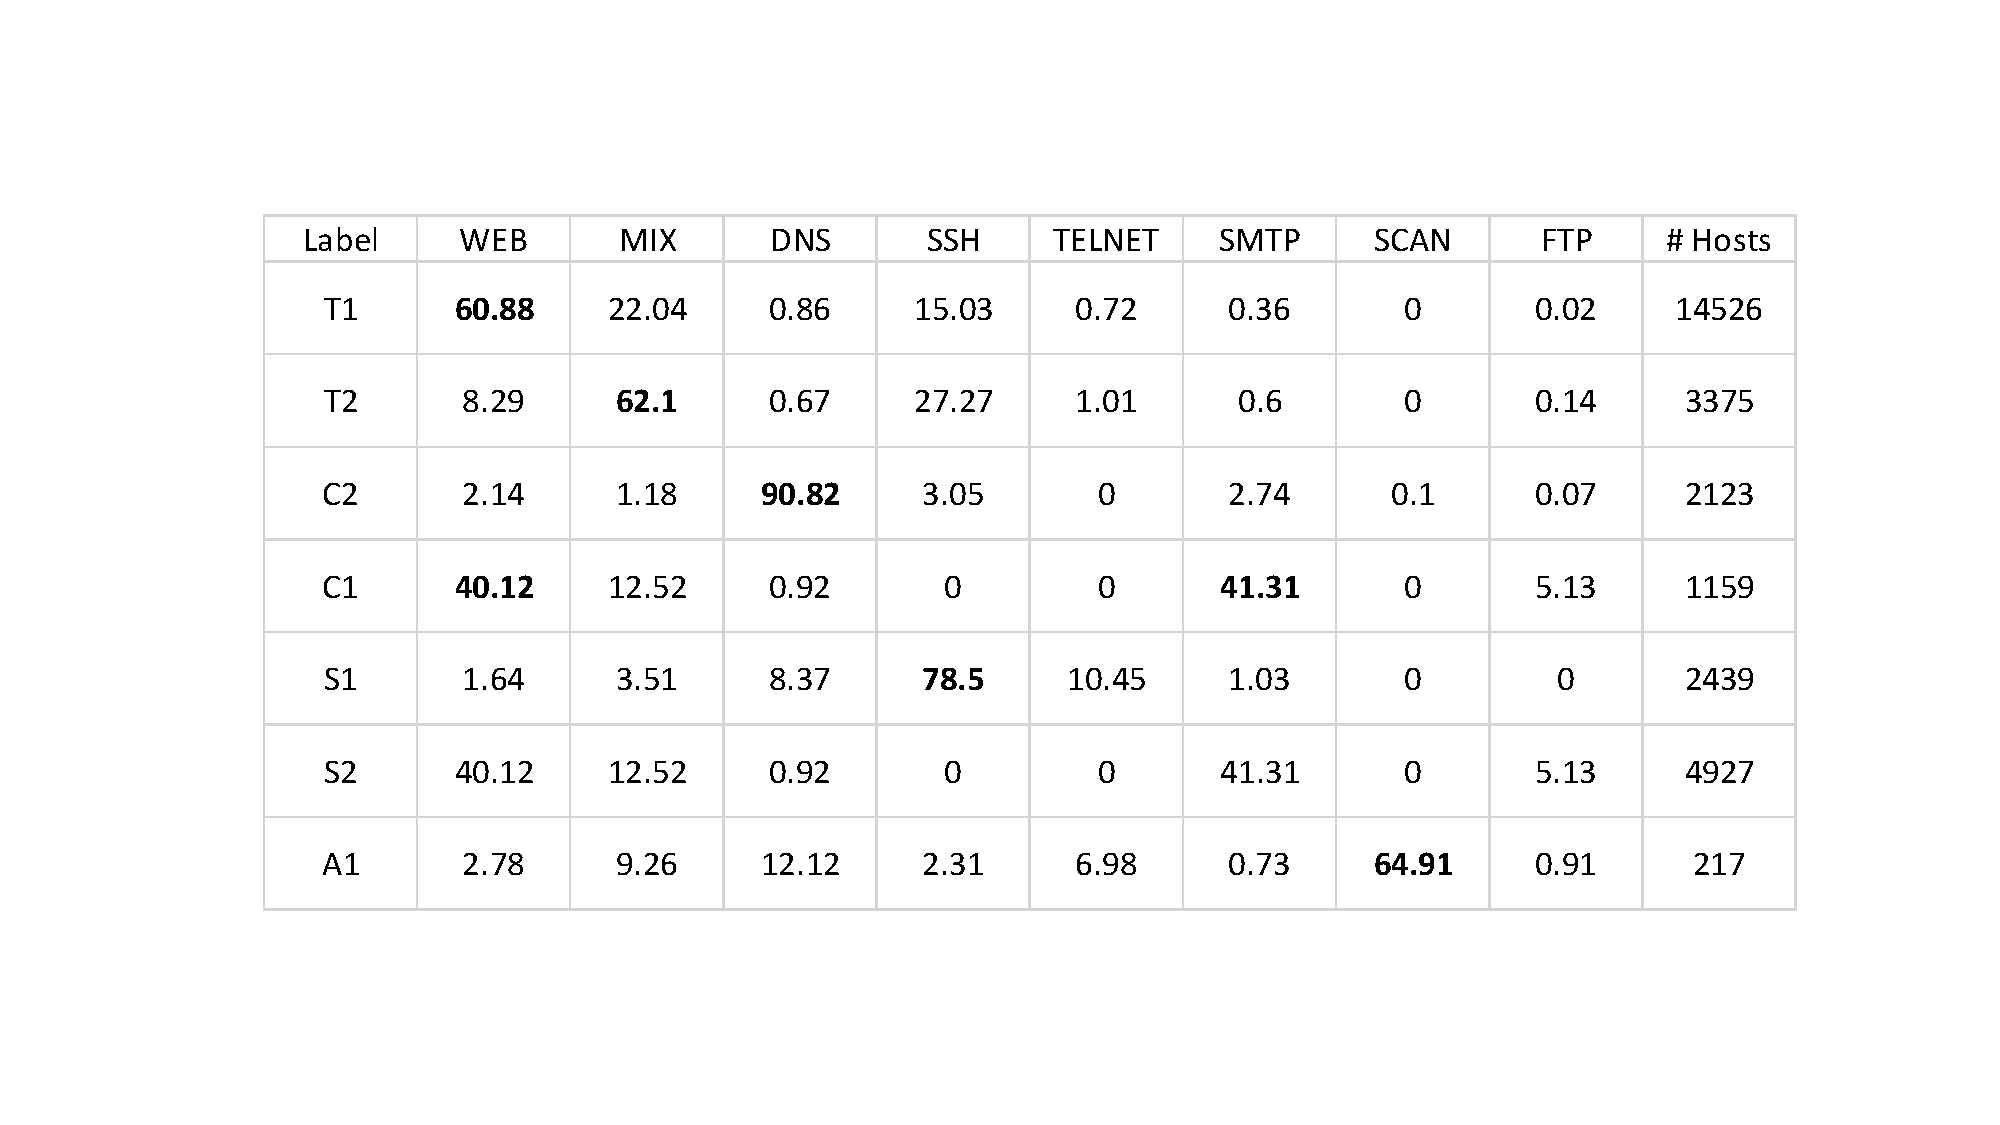
\includegraphics[scale = 0.5]{validation.pdf}}	
	\tablabel{validation}
\end{table}

The row headers in the table correspond to the lables of the clusters generated by our system while the column headers correspond to the different classes of traffic derived by a port based classifier as mentioned above. Each row in the table describes the percentage of hosts within each cluster that fall under different classes of traffic as classified by a port based classifier. For example, in the cluster T1 we have 60.88\% of hosts that are using web applications, 0.86\% of hosts are involved in DNS traffic, 15.03\% of hosts exchange SSH, 0.72\% exchange TELNET traffic and 22.04\% of the hosts in this cluster are classified as MIX traffic. Some important observations from this table are:

\begin{itemize}
	\item From the bolded parts in the table we can safely conclude that we have an high match of host classification which reflects the competence of the proposed procedure.
	
	\item  It is also clearly evident from here that the nature of clusters described earlier confirm with the results obtained with cross-validation.
	
	\item This also suggests that all the hosts that fall into a particular class based on port based analysis are not necessarily in the same cluster. They are dispersed across the clusters which shows the necessity of a host based behavior extraction.	
\end{itemize}
  For example, cluster S1 clearly confirms the fact that the hosts in this cluster are dealing with SSH traffic and the same traffic is also present in T1 and T2 clusters. Similary, hosts in the cluster S2 contains of servers that provide responses for web, ssh and other requests. This cluster has similar distribution as cluster C1 but they act exactly opposite like servers and clients respectively. Also, few points of observation from the table are, T1 has mostly requests and responses between hosts spread across different applications. hosts which are grouped as T2 have most of it's hosts labeled as Mix, which on further investigation revealed that many of the hosts in this class don't pass the majority test to be distinguished into any particular class. Finally, Scanners distribution was minimal across all the clusters. The sparsity of this table also serves as a confident measure for our proposed approach.

\section{Labeled Data: description and clustering}

In this section we are evaluating our system to determine its accuracy and precision on identifying host behaviors using labeled data. The labeled data that we used in this section is provided by Center for Applied Internet Data Analysis (CAIDA). CAIDA is a research group based at the San Diego Supercomputer Center (SDSC) on the UC San Diego campus who conduct network research and build research infrastructure to support data collection, and data distribution to the scientific research community.

CAIDAs dataset consists of thirteen different scenarios. Each scenario is a capture of network data written into a pcap file. Each capture consists of both real network traffic and the synthetic traffic they have generated to emulate that scenario. For our evaluation purpose we are considering four of these scenarios.

\begin{itemize}
	\item In the first scenario they have generated traffic to emulate the situation of scanners in the network and hence their capture consists of two classes of traffic namely,  Normal and Scanning web proxies.
	\item In the second scenario they have generated traffic to emulate the situation of chinese attackers in the network and hence their capture consists of two classes of traffic namely,  Normal and Chineses hosts.
	\item The third scenario consists of synthesized traffic to emulate DDOS attacks. Also, they have let the background traffic to mix with normal traffic. Hence, in total we have three classes of traffic namely, Normal, Background and UDP\& ICMP DDOS attacks.
	\item Fourth scenario consists of synthesized traffic to emulate a situation were multi-networks are interacting. 

\end{itemize}

 These scenarios are captured into pcap files which are further processed to obtain information about NetFlows. \tabref{synthdesc} represents the duration of each scenario and the contents of the pcap file such as the number of packets, the number of NetFlows and the size of the file itself. The distinctive character of this data set is that the data captured in each scenario is manually examined and labeled. The labeled dataset looks similar to the one which we capture at the emulab router excpet for the last column where the flow is labeled which can be seen in the \figref{ss_labeled}.


\begin{table}[t]
	\caption{Dataset description.}%
	\centerline{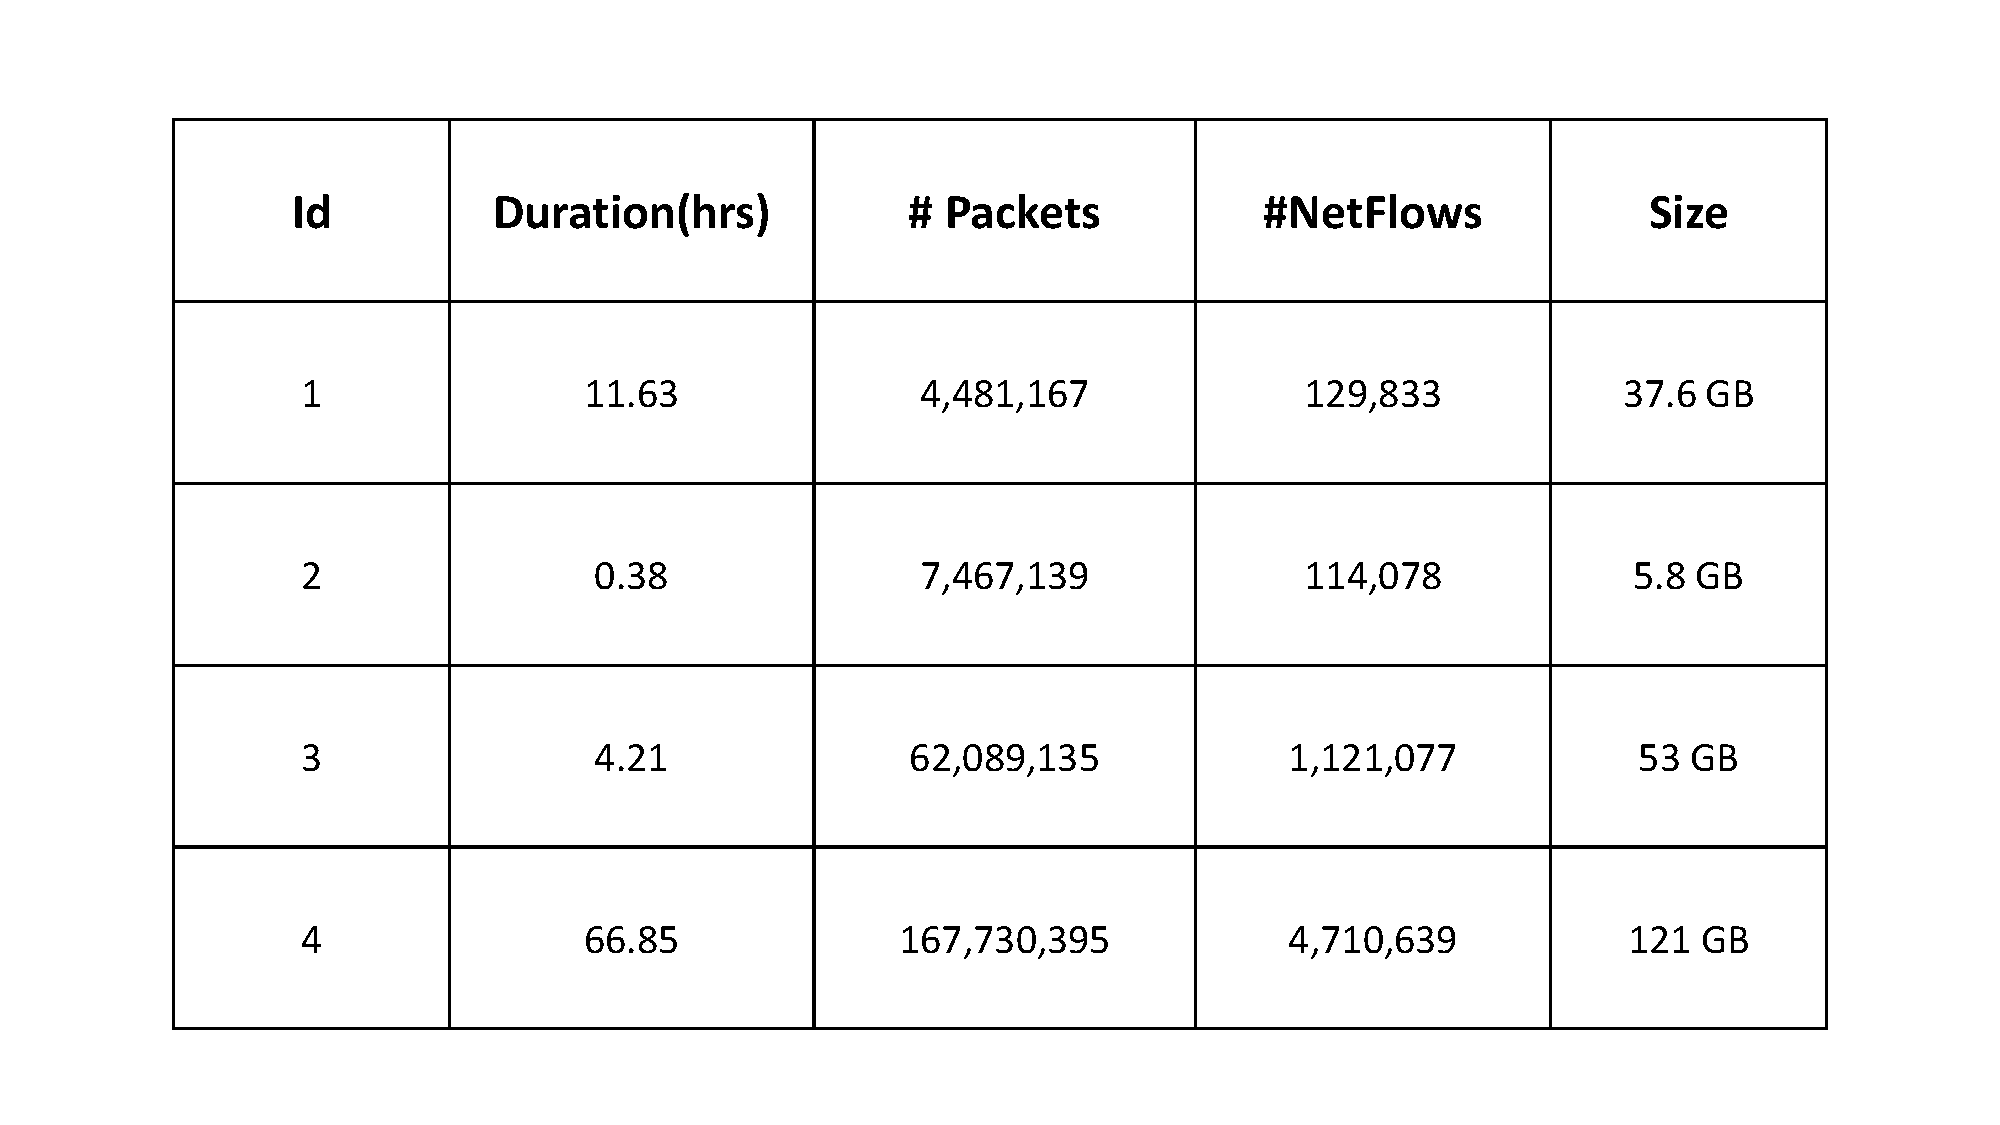
\includegraphics[scale = 0.5]{synth_desc.pdf}}	
	\tablabel{synthdesc}
\end{table}

\begin{figure}[t]
	\centerline{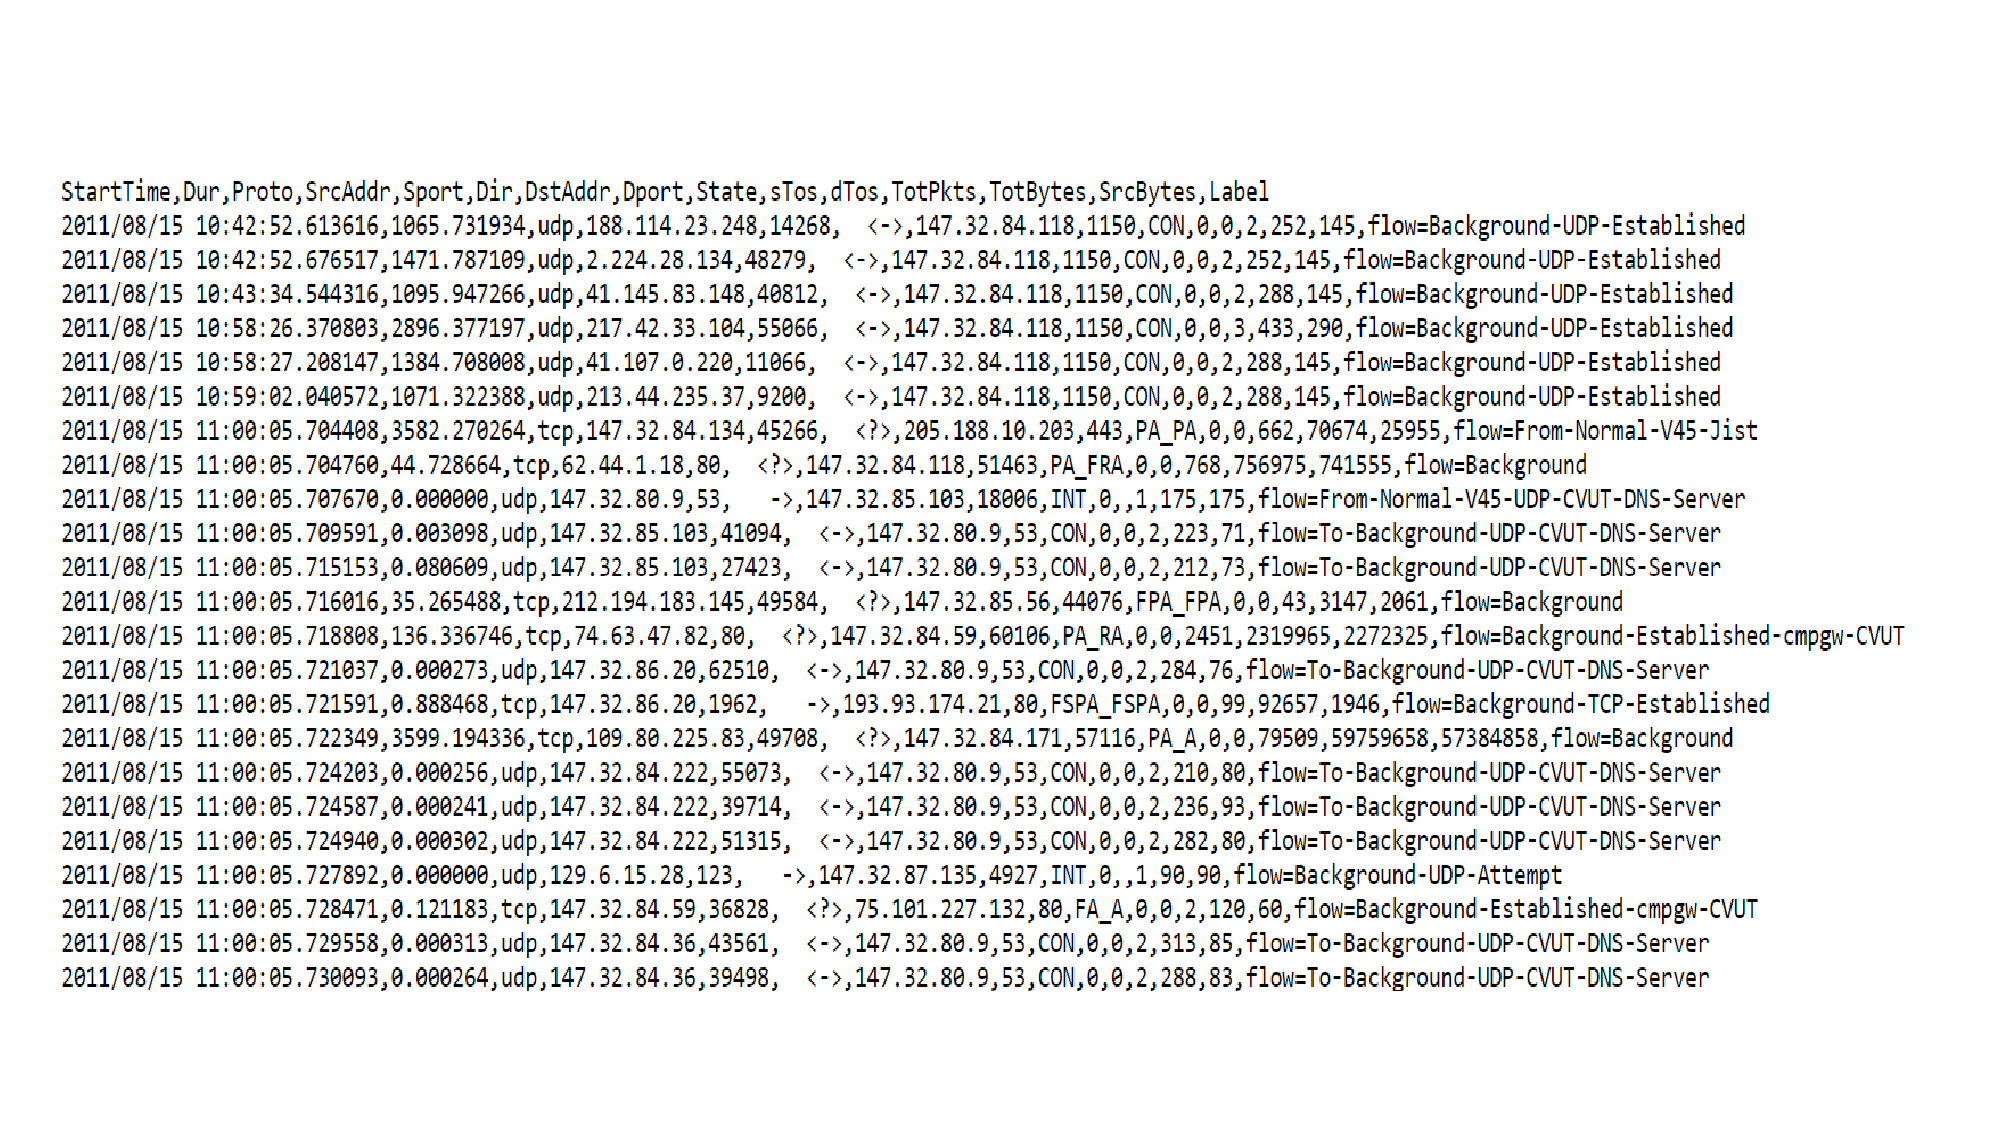
\includegraphics[trim=4cm 3cm 3cm 3cm, scale = 0.5]{ss_labeled.pdf}}
	\caption{Manually labeled dataset by CAIDA.}%
	\figlabel{ss_labeled}
\end{figure}

	

Using the different captures in \tabref{synthdesc}  we evaluated our systems basic functionality such as how effectively our system is able to extract the host behaviors, the detection rate of the different possible attacks and how will it respond with scale (when there are multiple hosts from multiple networks communicating simultaneously). Before looking into these results let us examine some basic terminology to understand the evaluations.

Let us consider a labeled dataset with two different labels A and B. The results produced when this dataset is sent through a classifier for classification can be tabulated as a confusion matrix as shown in \tabref{confusion}. This table tells us that datset cosists of a total of N values both of label A and label B combined. TPA indicates number of data points that are labeled as A and are classified as A. TPB indicates the number of data points that are labeled as B and are classified as B. EAB indicates the number of data points that are labeled as B by the classifier but actually belong to label A. EBA indicates the number of data points that are labeled as A by the classifier but actually belong to label B. The key of this matrix is the number of correct and incorrect classifications are summarized with count values and broken down by each class. The confusion matrix shows the ways in which a classification model is confused when it is making classifications. It also gives insights into the errors classifier is making and more importantly the type of errors that are being made. From this matrix we can calculate accuracy and prediction of a system which are defined as follows:

\begin{itemize}
	\item \textbf{Accuracy:} is calculated as the sum of correct classifications divided by the total number of classifications.
	\begin{center}
		\centering accuracy (A) = $ \frac{TPA + TPB}{N}$
	\end{center}
	 

	\item \textbf{Precision:} of a class is calculated as correct classifications divided by total number of classifications for the class in consideration.
	\begin{center}
		\centering precision (P) for class A = $ \frac{TPA}{TPA + EBA}$ \\
		\centering precision (P) for class B = $ \frac{TPB}{TPB + EAB}$
	\end{center}
	
	\item \textbf{Misclassification Rate:} is calculated as the sum of incorrect classifications divided by the total number of classifications.
	\begin{center}
		\centering Misclassification (M) = $ \frac{EAB + EBA}{N}$
	\end{center}
	
\end{itemize}

\begin{table}[b]
	
	\caption{Confusion Matrix}%
	\centerline{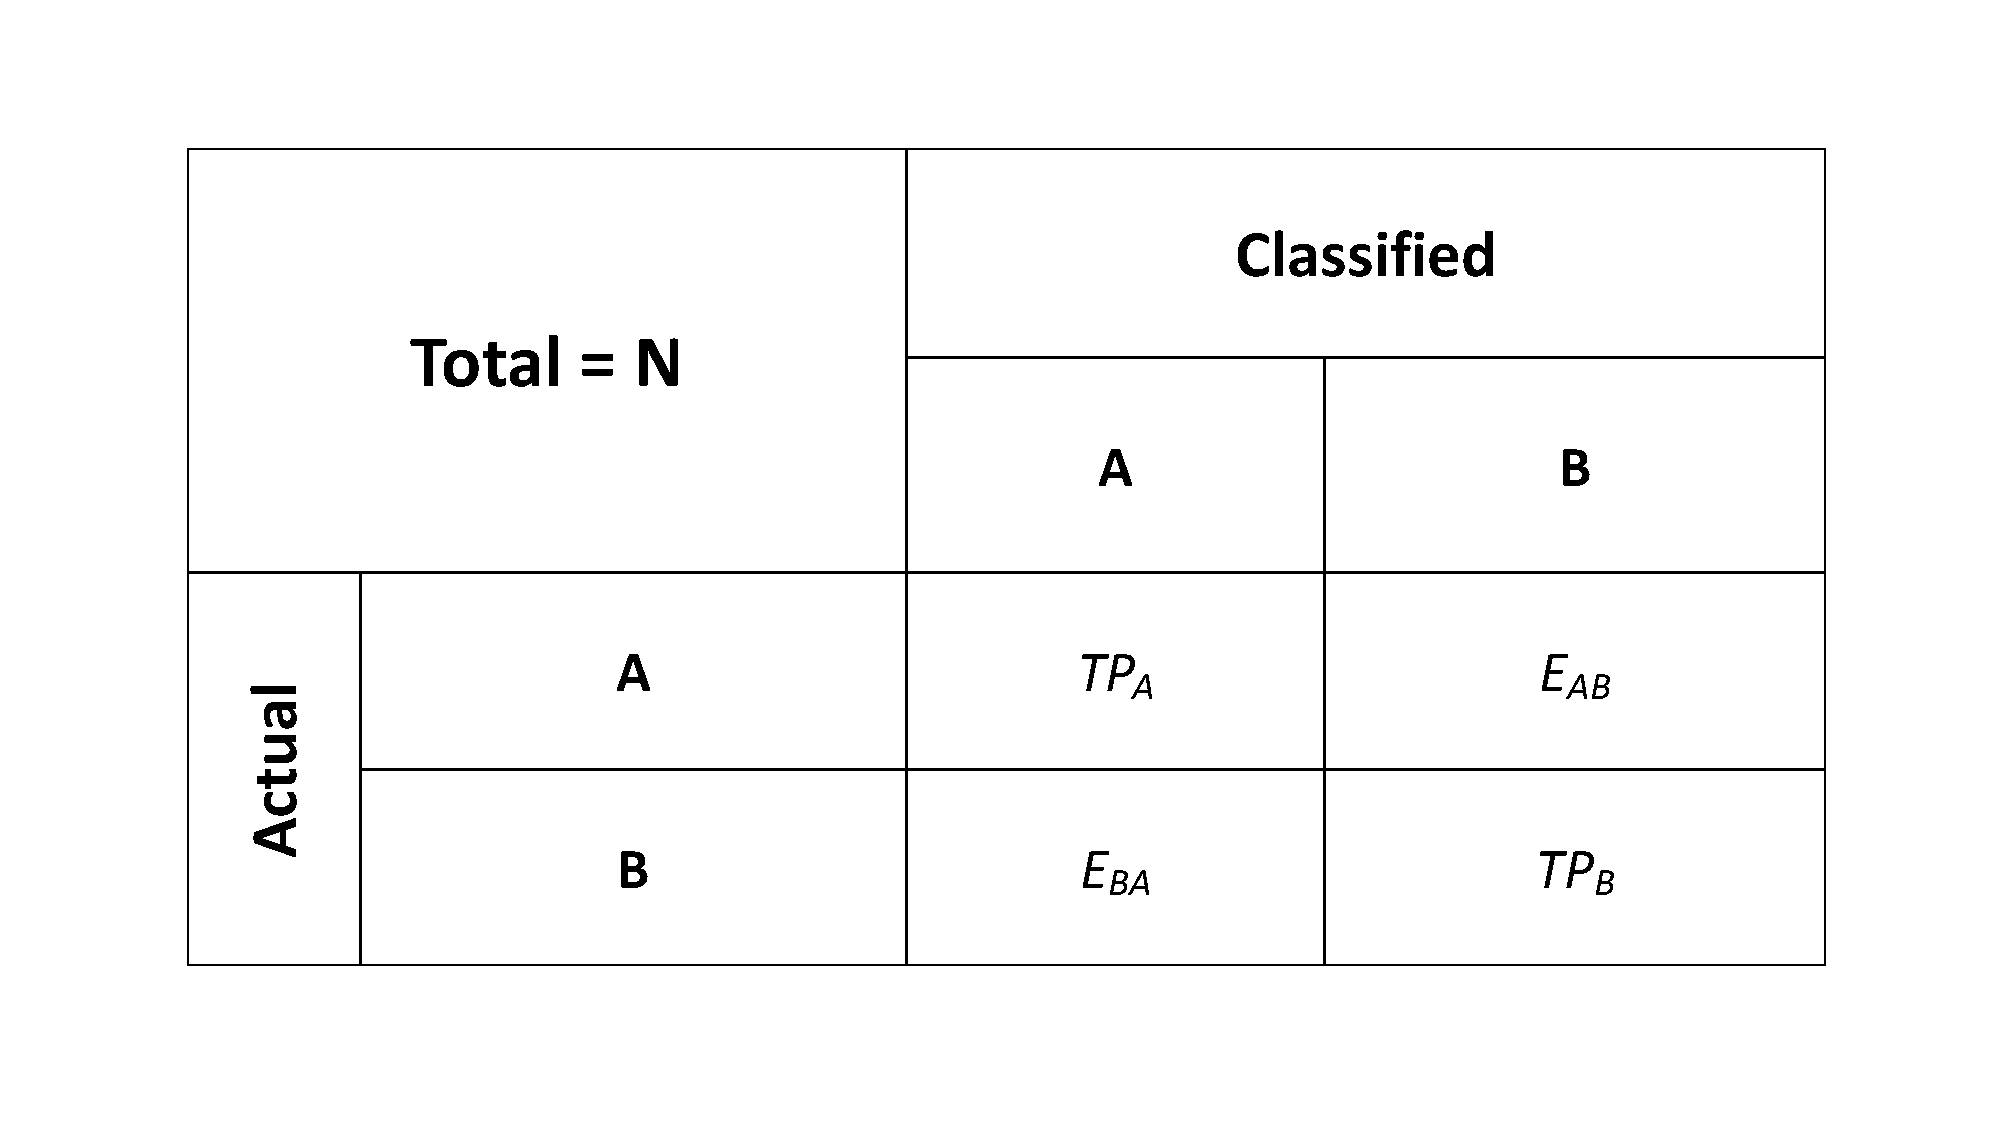
\includegraphics[scale = 0.5]{confusion.pdf}}	
	\tablabel{confusion}
\end{table}
On similar lines the confusion matrix can be extended to any number of classes and can be useful in calculating different performance numbers of this system. One important point to note here is when we pass this labeled dataset through our system we get clusters contrary to a classifier which gives a label for each data point. Inorder to circumvent this issue we look at the clusters and label them. If a cluster is dominated by any particular label we retain the label for that cluster and the other clusters are named according to the manual inspection. After this process the results obtained are as below. 



\subsection{Scenario 1:}
The scenario 1 is of duration 11.63 hours with 37.6 GB of data. This dataset contains hosts exhibiting two unique behaviors namely normal traffic and scanners. Through this experiment we would like to check our systems basic functionality of identifying different behaviors. When we passed this data through our sytsem we found formation of two major clusters each dominated by a label and hence we retained the labels for these clusters as mentioned above. The results are as shown in  \tabref{scenario1}. 



\begin{itemize}
	\item \textbf{Accuracy:} (42503+80252)/129833 = 94.54\%
	
	\item \textbf{Misclassification Rate:} (3987+3091)/129833 = 5.45\%
	\item \textbf{Precision:} 
	\begin{itemize}
		
				
		\item (42503)/46490 = 91.4\% precise in finding scanners.
		
		\item (80252)/83343 = 96.2\% precise in finding normal hosts.
			
	\end{itemize}

\end{itemize}
\begin{table}[t]
	\caption{Scenario 1.}%
	\centerline{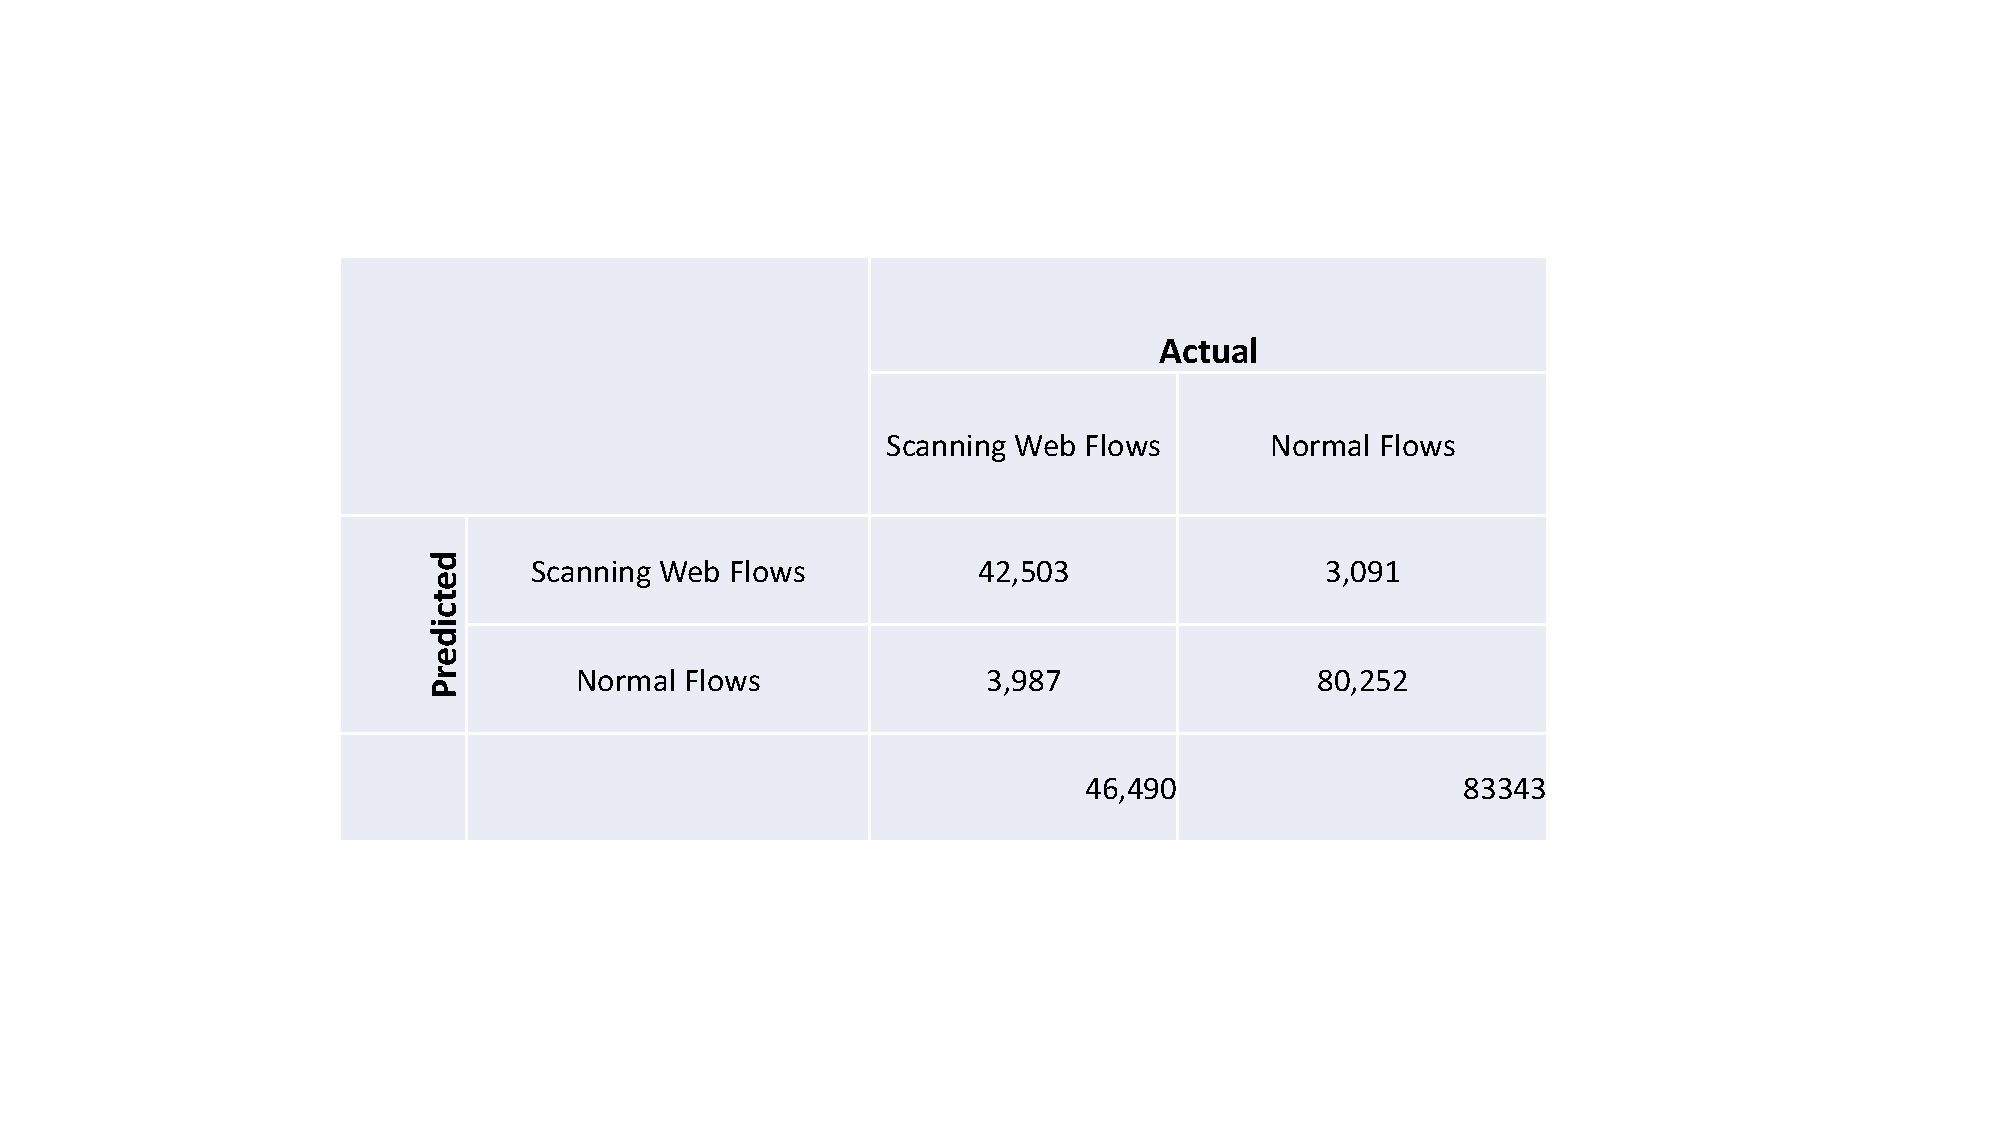
\includegraphics[scale = 0.5]{scenario1.pdf}}	
	\tablabel{scenario1}
\end{table}

From this we learn that our system can identify unique behaviors with high accuracy and precision.

\subsection{Scenario 2:}
The scenario 2 is of duration 0.38 hours with 5.8 GB of data. This dataset contains hosts exhibiting two unique behaviors namely normal traffic and chinese hosts. This experiment is aimed to determine the basic functionality of our system as scenario 1 and to determine the rate of detection of chinese hosts which are prevalent in our real data set collected at Emulab routers. When we passed this data through our system we found formation of two major clusters each dominated by a label and hence we retained the labels for these clusters and the results are as shown in \tabref{scenario2}.

\begin{table}[b]
	\caption{Scenario 2.}%
	\centerline{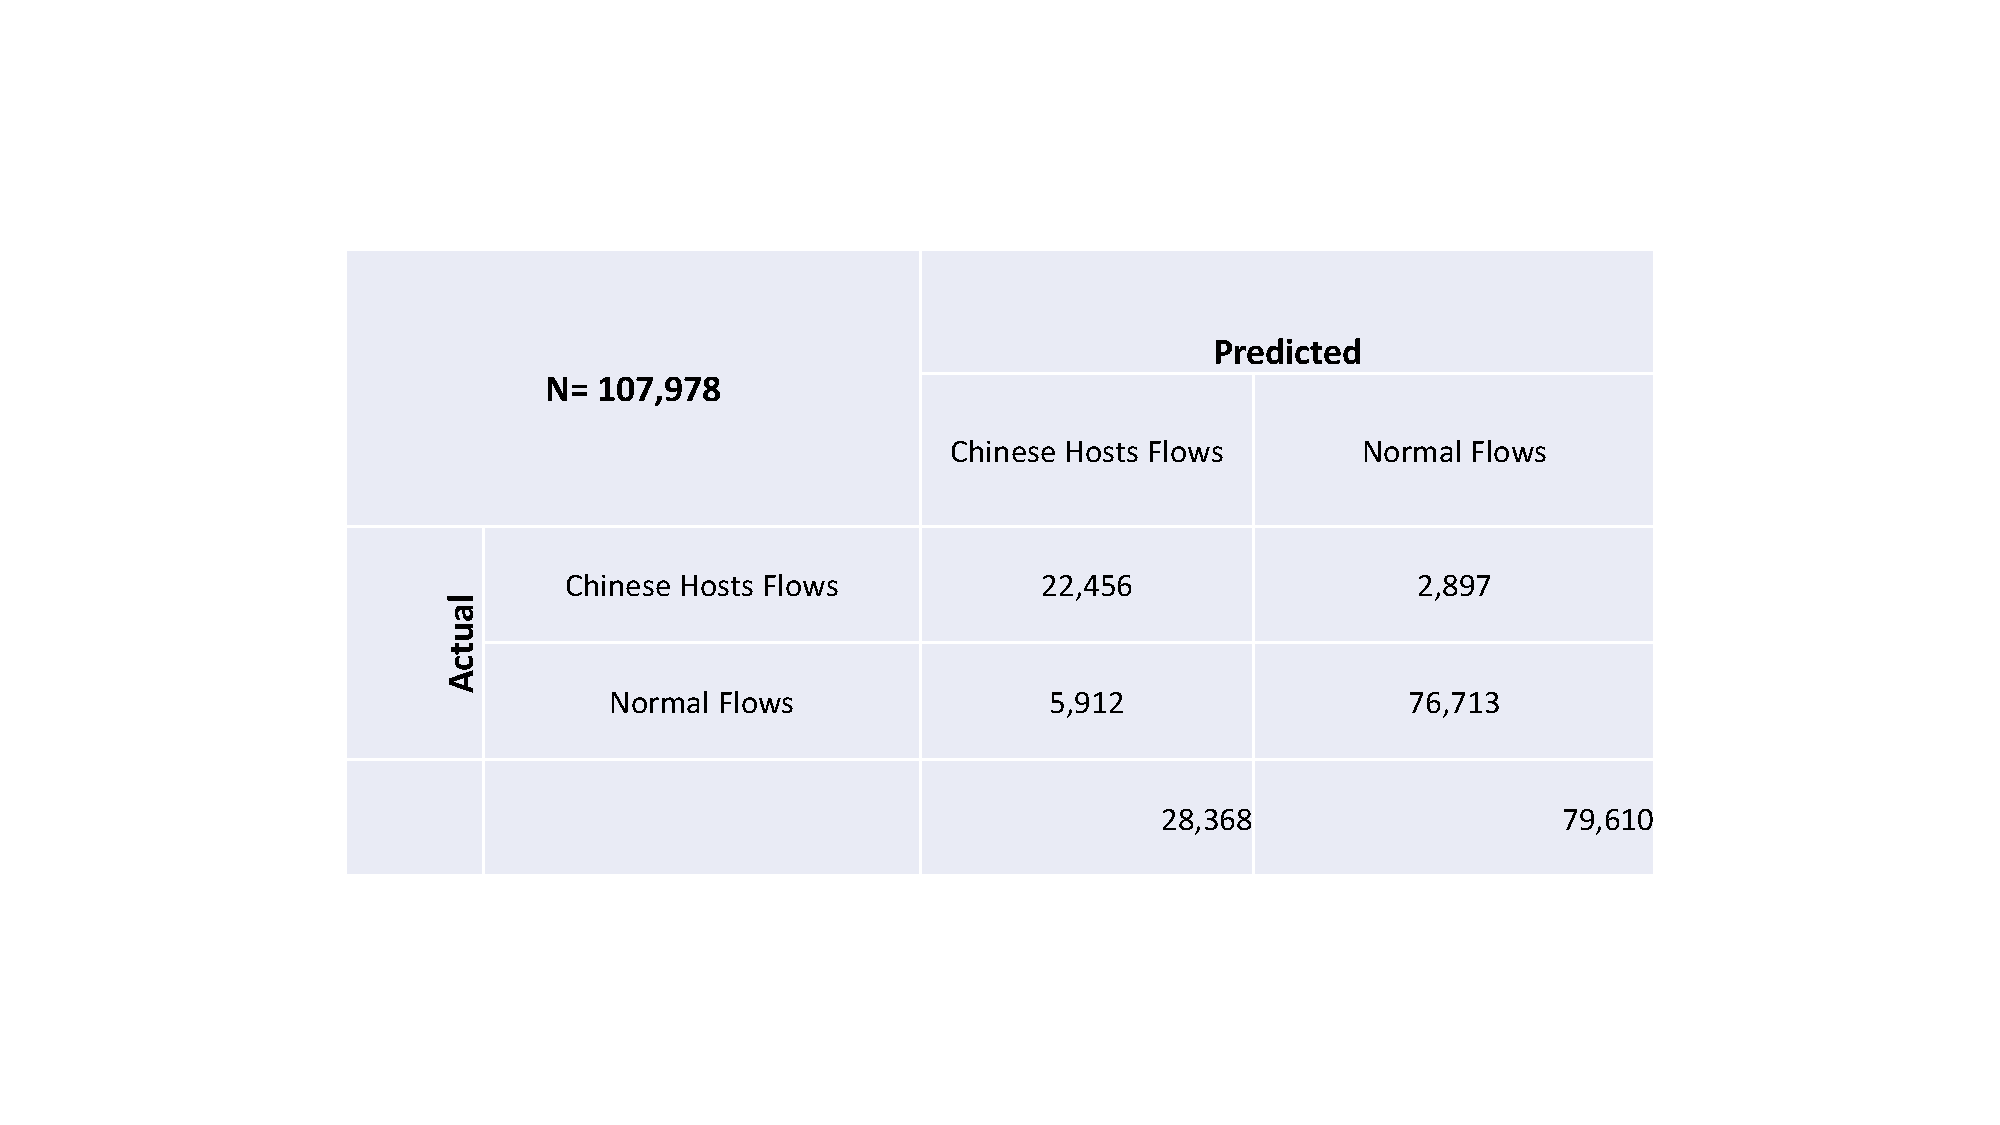
\includegraphics[scale = 0.5]{scenario2.pdf}}	
	\tablabel{scenario2}
\end{table}

\begin{itemize}
	\item \textbf{Accuracy:}  (22456+76713)/107978 = 89.18\%
	
	\item \textbf{Misclassification Rate:} (5912+2897)/107978 = 11.7\%
	
	\item \textbf{Precision:} 
	\begin{itemize}	
			
		\item (22456)/28368 = 76.1\% precise in finding chinese hosts.
		
		\item (76713)/79610 = 96.3\% precise in finding normal hosts.
		
	\end{itemize}
	
\end{itemize}

This experiment confirms that our system does well in distinguishing normal hosts but fairs poorly in identifying chinese hosts.

\subsection{Scenario 3:}
The scenario 3 is of duration 4.21 hours with 53 GB of data. This dataset contains hosts exhibiting three unique behaviors namely normal, background, UDP \& ICMP DDOS  traffic. This experiment is aimed to determine the functionality of our system in face of adversory attacks and mutliple types of traffic. When we passed this data through our system we found formation of three major clusters each dominated by a label and hence we retained the labels for these clusters and the results are as shown in \tabref{scenario3}.

\begin{table}[t]
	\caption{Scenario 3.}%
	\centerline{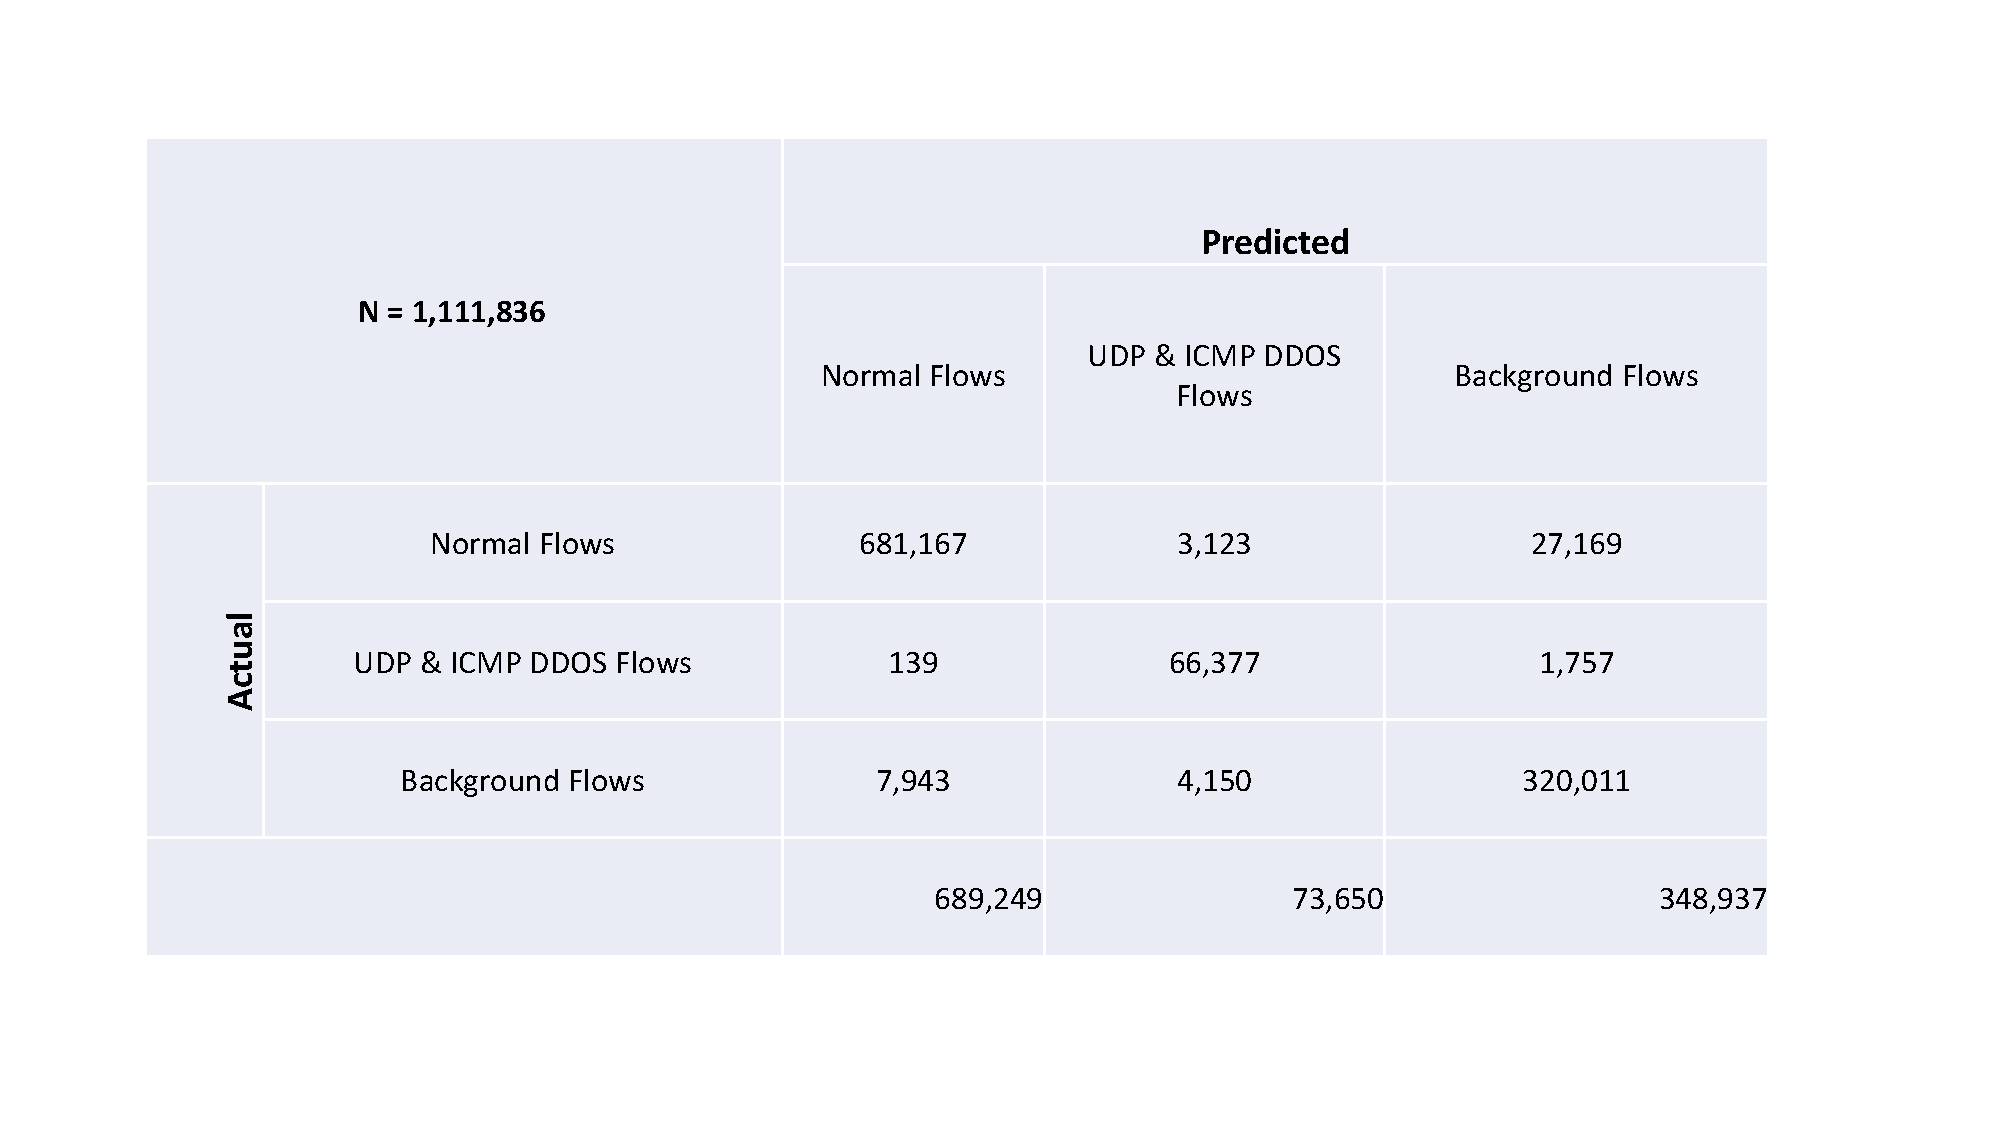
\includegraphics[scale = 0.5]{scenario3.pdf}}	
	\tablabel{scenario3}
\end{table}

\begin{itemize}
	\item \textbf{Accuracy:}  (681167+66377+320011)/1111836 = 96.01\%
	
	\item \textbf{Misclassification Rate:} (3123+27169+139+1757+7943+4150+2897)/1111836 = 3.98\%
	
	\item \textbf{Precision:} 
	\begin{itemize}	
		
		
		\item (681167)/689249 = 98.8\% precise in finding hosts pertaining to normal traffic.
		
		\item (66377)/73650 = 91.17\% precise in finding background hosts.
		
		\item (320011)/348937 = 90.23\% precise in finding UDP \& ICMP DDOS hosts.
		
	\end{itemize}
	
\end{itemize}

\subsection{Scenario 4:}
The scenario 4 is of duration 66.85 hours with 121 GB of data. This dataset contains hosts exhibiting multiple behaviors namely normal, background, UDP \& ICMP DDOS, HTTP, Port Scan, DNS and Fast Flux traffic. This experiment is aimed to determine the functionality of our system in a complex network scenario where we see multiple behaviors. When we passed this data through our system we found formation of seven major clusters, interestingly the labeled dataset also exhibits seven different behaviors. When we looked at these clusters six of them are dominated by a label and hence we retained the labels for these clusters where as the last cluster didn't have any majority label and hence we labeled it by inspection as Heavy Hitters. cluster  results are as shown in \tabref{scenario4}.

\begin{table}[t]
	\caption{Scenario 4.}%
	\centerline{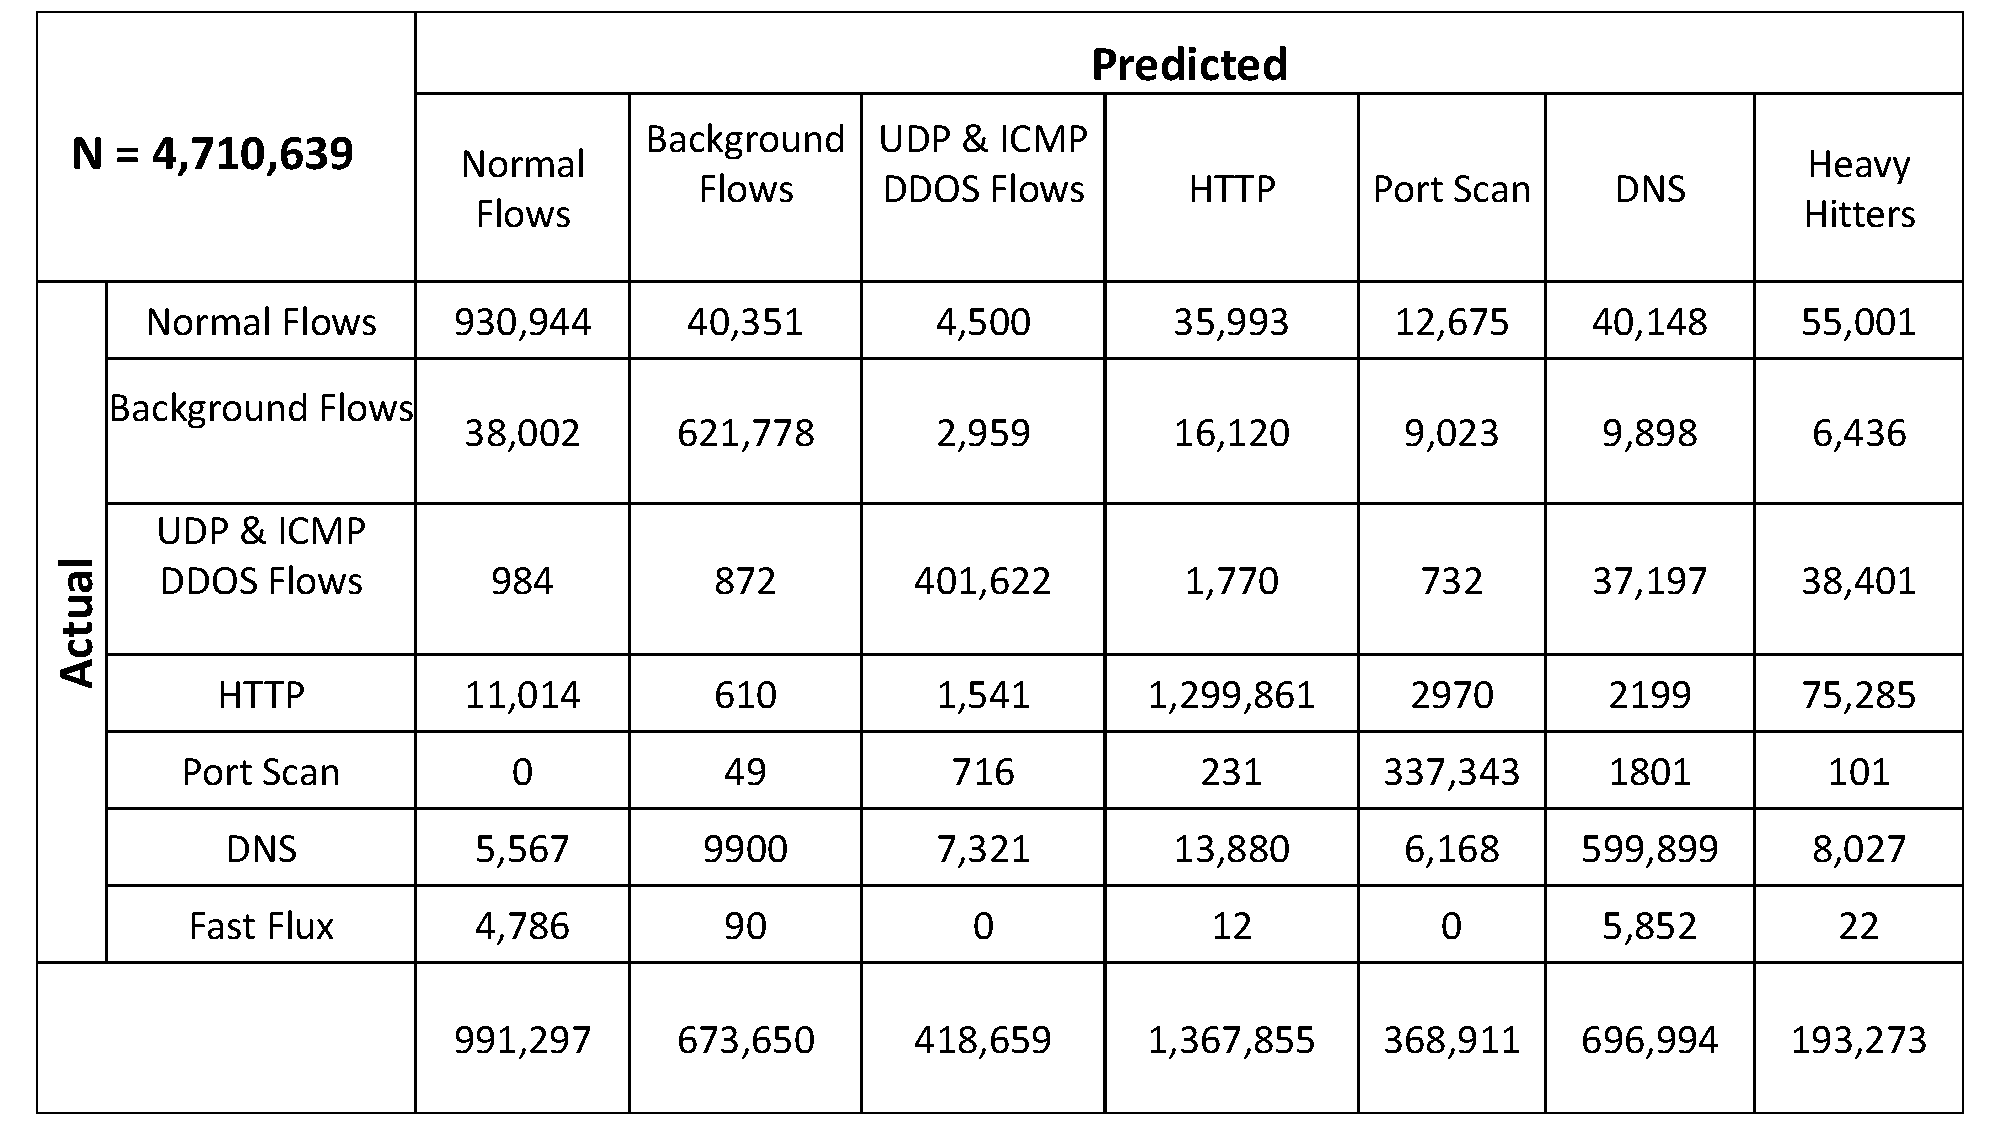
\includegraphics[scale = 0.5]{scenario4.pdf}}	
	\tablabel{scenario4}
\end{table}

\begin{itemize}
	\item \textbf{Accuracy:}  (930944+621778+401622+1299861+337343+599899)/4710639 = 89.78\%
	
	\item \textbf{Misclassification Rate:} (518170)/4710639 = 10.22\%
	
	\item \textbf{Precision:} 
	\begin{itemize}			
		
		\item (930944)/991297 = 93.9\% precise in finding hosts pertaining to normal traffic.
		
		\item (621788)/673650 = 92.3\% precise in finding background hosts.
		
		\item (401622)/418659 = 91.23\% precise in finding UDP \& ICMP DDOS traffic.
		
		\item (1299861)/1367855 = 95.23\% precise in finding HTTP traffic.
		
		\item (337343)/368911 = 91.4\% precise in finding UDP \& ICMP DDOS hosts.
		
		\item (599899)/696994 = 86.06\% precise in finding DNS traffic.
	\end{itemize}
	
\end{itemize}

Our system was unable to detect the hosts exhibitng Fast Flux behavior on the other hand it grouped hosts which are transferring heavy payload across all the different labeled behaviors. We believe there are certain areas that our system has to focus on when it comes to grouping hosts in multiple networks.


\subsection{Hosts behavior with time:}

To determine the change in hosts behaviors over time we passed six months worth of data through our system similar to the experimental set up mentioned at the start of evaluation section. But this time we also invoked the method to calculate K value on every day. The K value determines the different behaviors the hosts are exhibitng on that day as mentioned in section \ref{cluster_labeling}. So, we have K unique behaviors on every day. We wanted to verify how this K value is changing with time. i.e, how are the behaviors changing with time. Hence, we plotted the K values for the last six months and it looks as follows \figref{constant}. The value of K on X-axis and the day on which we found this value on Y-axis. Except for few points it is a straight line indicating the constant behaviors that hosts are exhibiting in our system. This needn't be the case with all the networks. In an environment with multiple networks the K value could be differnt and we might see it changing frequently. It depends on the environment in which our system is going to be used.

\begin{figure}[t]
	\centerline{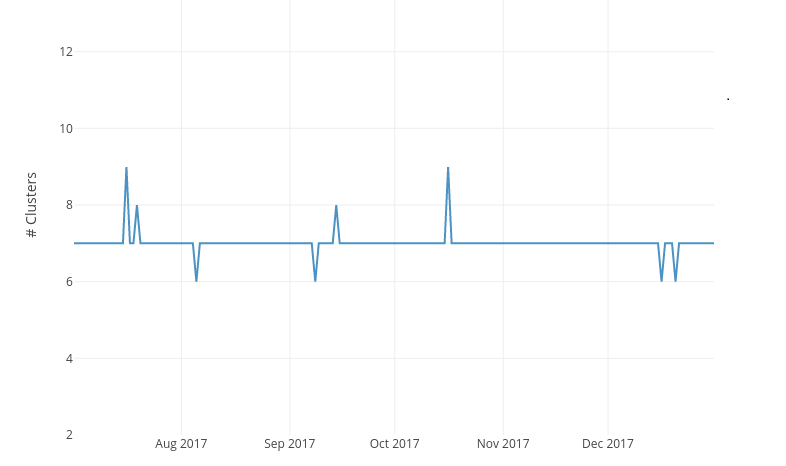
\includegraphics{constant.png}}
	\caption{ Plot of number of clusters formed over a time period.}%
	\figlabel{constant}
\end{figure}




\subsection{Applications:}

 As mentioned in section \ref{applications} our system can be used to build different applications that are helpful in network management. In that direction we have built a web tool to analyze these host behaviors. Our web tool collects the information from the pattern detection process such as cluster centers, labels etc.. and renders different visualizations.
 
 \begin{itemize}
 	\item \figref{compare_days} is a screenshot of the web tool. Left nav bar provides different options to exploarate the output produced by our system. In \figref{compare_days} we can see a comparison of host behaviors on two different days.
 	
 	\item The figure \figref{compare_weeks} gives an insight of how hosts behavior is changing over a month.
 	In the graph each line represents different host behaviors. The X-axis and Y-axis
 	represent the date on which this host behavior is observed and the number of hosts
 	which exhibited this behavior respectively.
 	
 \end{itemize}
 
 
\begin{figure}[t]
	\centerline{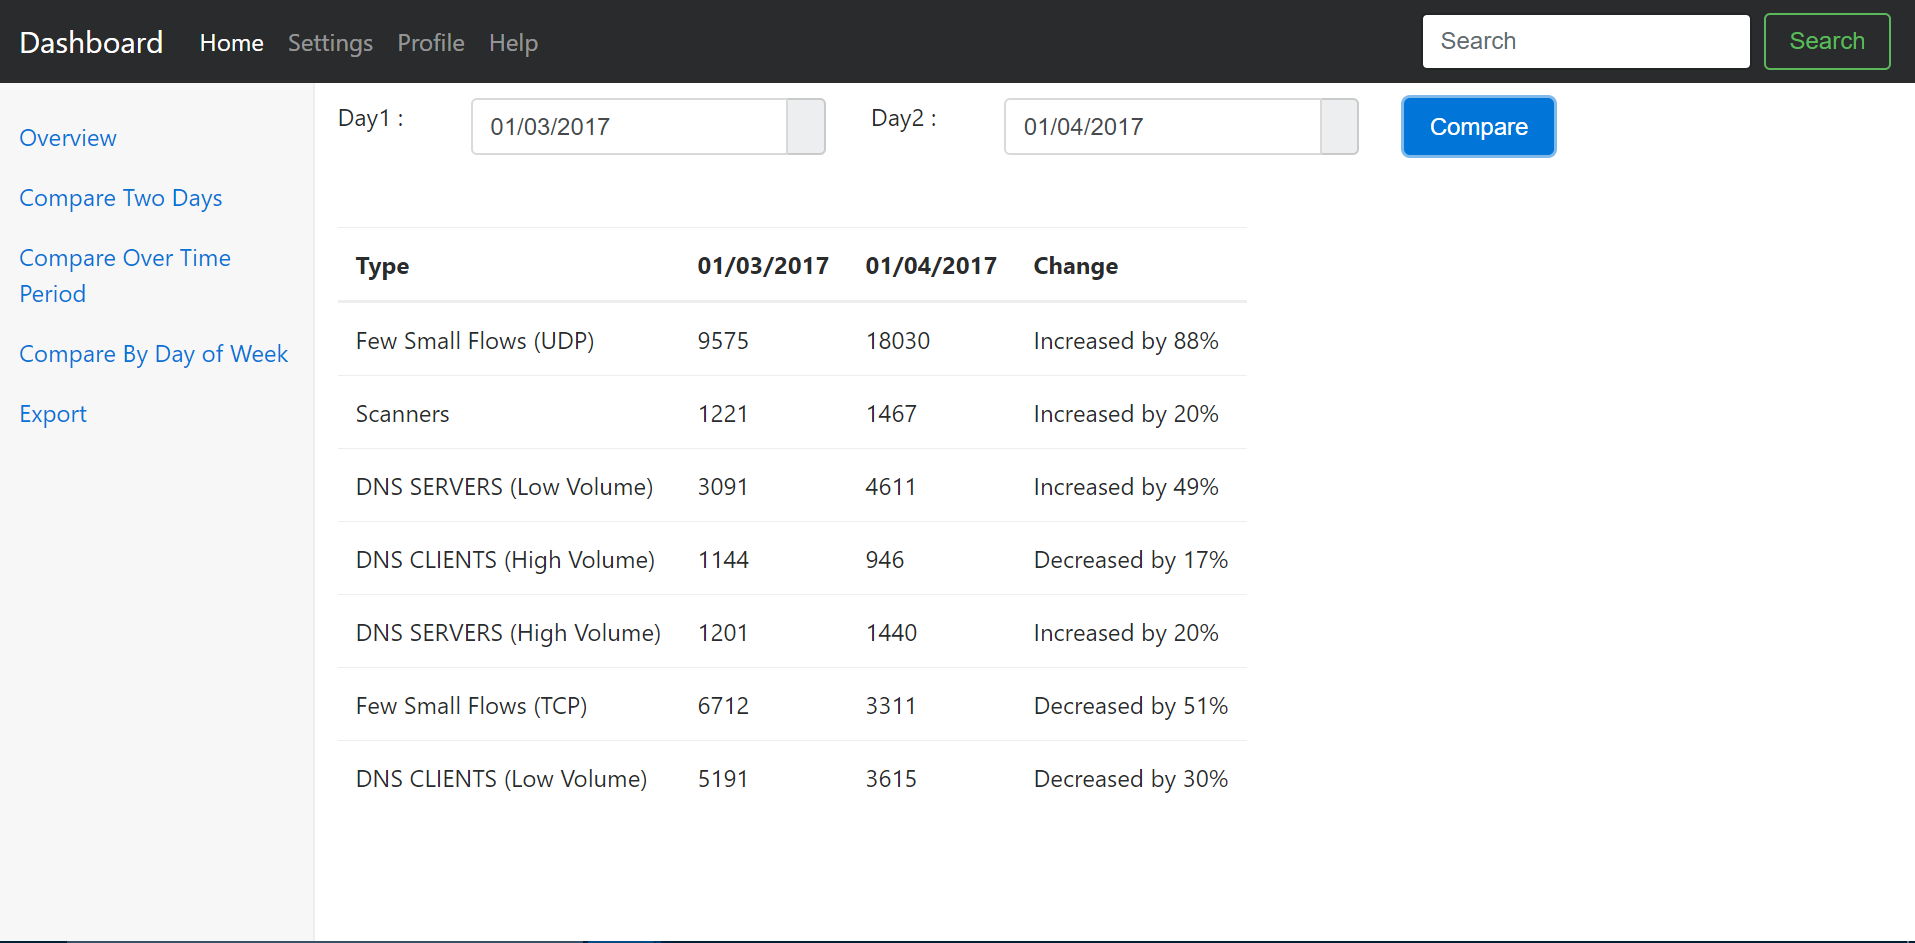
\includegraphics[scale = 0.45]{tool_compare_days.png}}
	\caption{Compare Host Behaviors on two days.}%
	\figlabel{compare_days}
\end{figure} 


\begin{figure}[t]
	\centerline{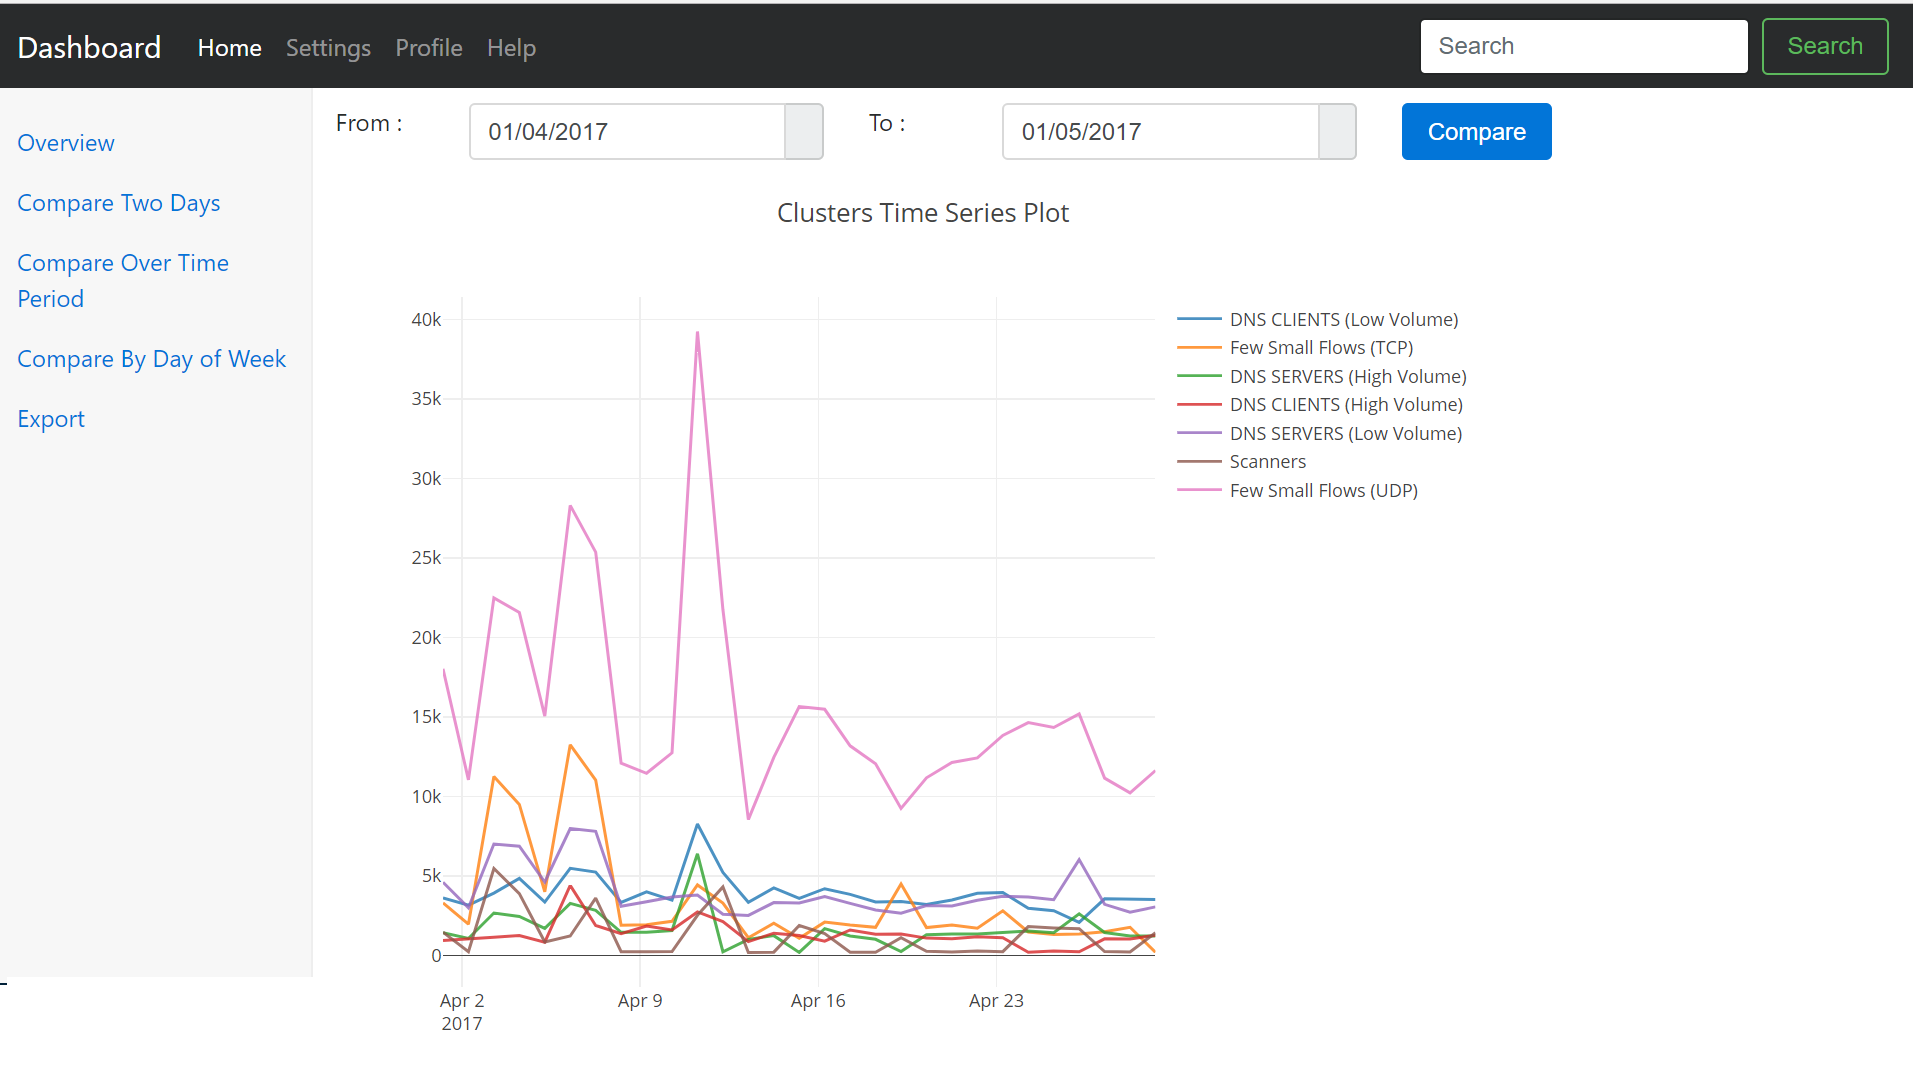
\includegraphics[scale = 0.45]{tool_compare_week.png}}
	\caption{Compare Host Behaviors over a time period.}%
	\figlabel{compare_weeks}
\end{figure}